\documentclass[11pt]{article}
    \usepackage{amsmath}
    \usepackage[pdftex]{graphicx}
    %\usepackage[usenames,dvipsnames,svgnames,table]{xcolor}
    \usepackage{amsmath,amsthm,amssymb,color,wrapfig,floatflt,amsfonts,listings,fancyhdr}
    \usepackage[parfill]{parskip}
    %\pagestyle{plain}
    \setlength\topmargin{.1cm}
    %\setlength\textheight{8in}
    \setlength\oddsidemargin{.1in}
    \setlength\evensidemargin{.1in}
    \setlength\textwidth{6.51in}
    %\setlength\headheight{52.5pt}
    \usepackage{fancyhdr}
    \usepackage[algosection, boxruled, linesnumbered]{algorithm2e}
    \pagestyle{fancy}
    \lhead{Arvind Ramaswami}
    \rhead{HW1}
    \chead{CS 4641 Machine Learning}
    \lfoot{}
    \cfoot{Page {\thepage}}
    \rfoot{}
    \newcommand{\RR}{\mathbb{R}}
    \newcommand{\CC}{\mathbb{C}}
    \newcommand{\HH}{\mathbb{H}}
    \newcommand{\BB}{\mathbb{B}}
    \newcommand{\ZZ}{\mathbb{Z}}
    \newcommand{\QQ}{\mathbb{Q}}
    \newcommand{\NN}{\mathbb{N}}
    \newcommand{\cP}{\mathcal{P}}
    \renewcommand{\And}{\wedge}
    \newcommand{\Or}{\vee}
    \newcommand{\Implies}{\Rightarrow}
    \newcommand{\Not}{\sim}
    \begin{document}
        \section{Classification problems}
            \subsection{Pima Indians Diabetes Dataset}

            This classification problem involves predicting whether or not a person has diabetes
            based on certain features.

            The features are: Pregnancies, Glucose, BloodPressure, SkinThickness, Insulin, BMI, DiabetesPedigreeFunction, Age.

            The dataset has 768 entries.

            This classification problem is interesting since it is not necessary
            clear whether someone has diabetes given those limited features, so there
            is not necessarily a clearly separable boundary. Running different algorithms
            in this problem should give some insight on how to find a proper boundary for
            such a dataset.

            \subsection{Predicting whether mushrooms are edible}

            The objective of this classification problem is to predict
            whether or not a mushroom is edible or poisonous, based on a set
            of given features.

            The features are: cap-shape, cap-surface, cap-color, bruises, odor, gill-attachment, gill-spacing, gill-size, gill-color, stalk-shape, stalk-root, stalk-surface-above-ring, stalk-surface-below-ring, stalk-color-above-ring, stalk-color-below-ring, veil-type, veil-color, ring-number, ring-type, spore-print-color, population, habitat

            The dataset contains 8,124 data points in total.


        
        \section{Results}

        The data was split into a training set, validation set, and testing set. The validation set consisted of 10% of the entire dataset, and the testing set consisted of 60% of the entire testing set. Below are plots that resulted from the scripts that were run.

    The training set size was varied, and for each training set size, the hyperparameters were those such that the accuracy on the validation set was maximized (For example, for a training set of size 5000, if the accuracy on the validation set of the decision tree was the highest when the max depth was 10 as opposed to max depths of 1, 2, 5 or 20, then the plotted accuracy for a training set of size 5000 would represent that of a max depth of 10).

    For iterative algorithms (The SVM and neural network), plots after certain numbers of iterations are included (this was done by testing multiple restrictions on the maximum number of iterations of the algorithm $--$ the max$\_$iter parameter in sklearn).


        \subsection{Decision Trees}
        The pruning used for the decision trees was caused by setting a limit on the maximum depth.

        Here are the plots:

        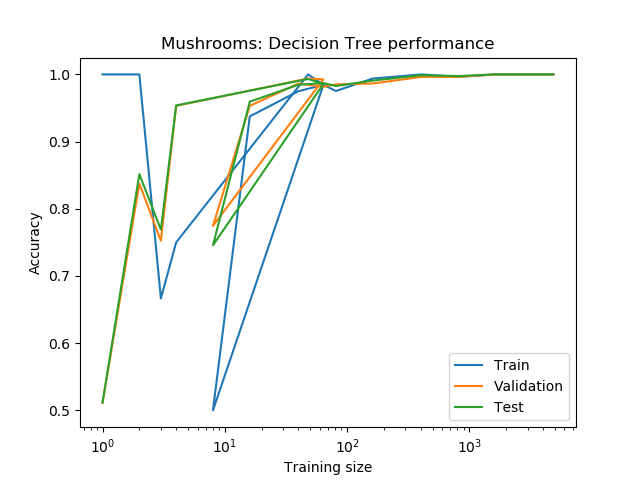
\includegraphics[width=8cm]{mushrooms/mushroom_dt_trainingsize.png}
        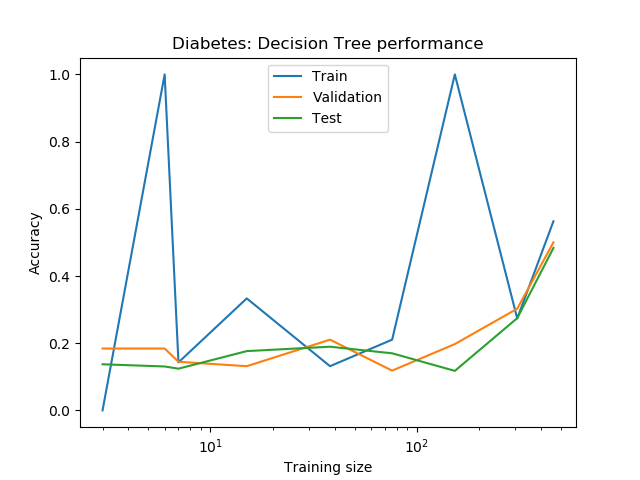
\includegraphics[width=8cm]{diabetes/diabetes_dt_trainingsize.png}

        \subsection{Neural Networks}

        Neural networks were tested with multiple combinations of layers.

        Below are the plots:

        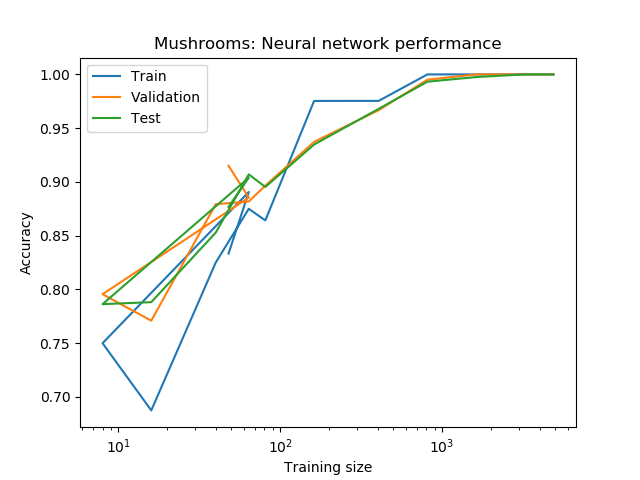
\includegraphics[width=8cm]{mushrooms/mushroom_nn_trainingsize.png}
        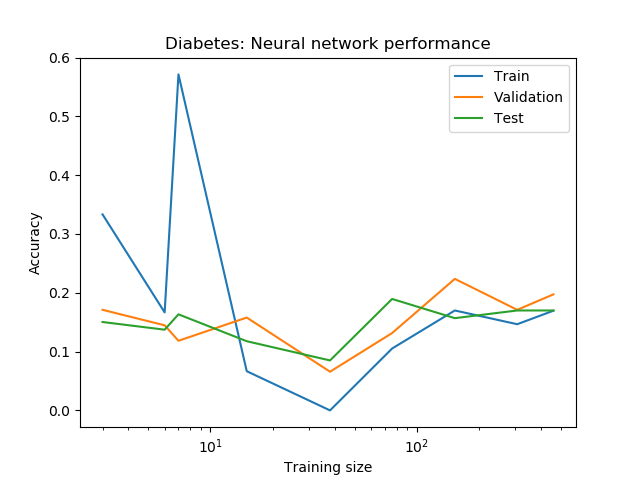
\includegraphics[width=8cm]{diabetes/diabetes_nn_trainingsize.png}

        Here are plots that represent the accuracy with respect to the number of iterations(done with the default sklearn parameters of 1 layer with 100 hidden units):

        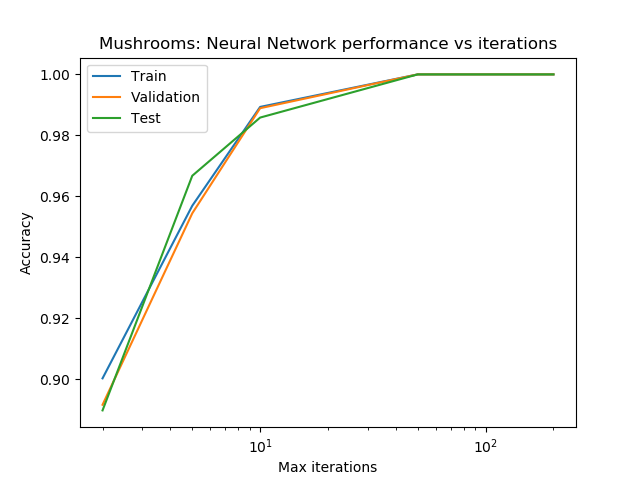
\includegraphics[width=8cm]{mushrooms/mushroom_nn_iterations.png}
        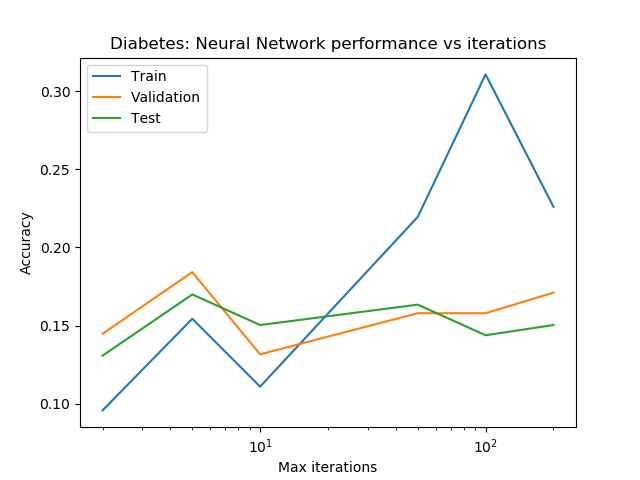
\includegraphics[width=8cm]{diabetes/diabetes_nn_iterations.png}

        \subsection{Boosting}
        The experiments in this project used an AdaBoost classifier with a base estimator of decision trees.
        The max depth of the decision trees (for sake of pruning) and the number of trees (base estimators)
        in the boosted classifier were varied.

        Here are the plots taken for boosting:

        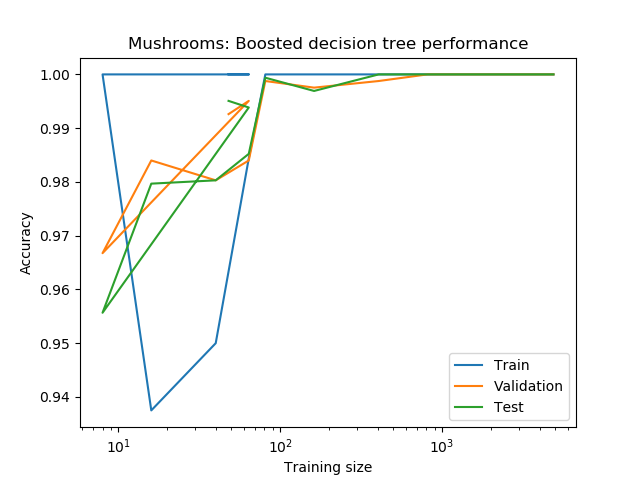
\includegraphics[width=8cm]{mushrooms/mushroom_boost_trainingsize.png}
        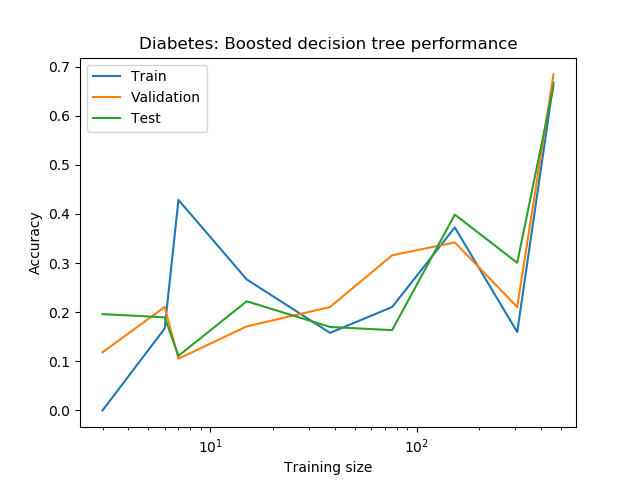
\includegraphics[width=8cm]{diabetes/diabetes_boost_trainingsize.png}

        \subsection{Support Vector Machines}
        The Support Vector Machines were tested with the linear kernel function and the RBF kernel function.

        The SVM plots are shown below:

        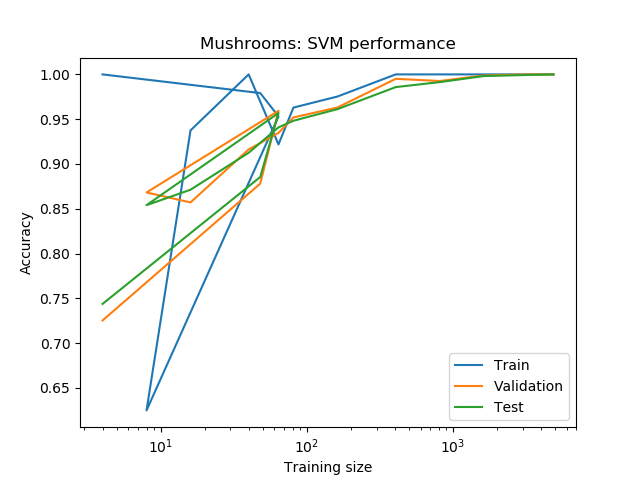
\includegraphics[width=8cm]{mushrooms/mushroom_svm_trainingsize.png}
        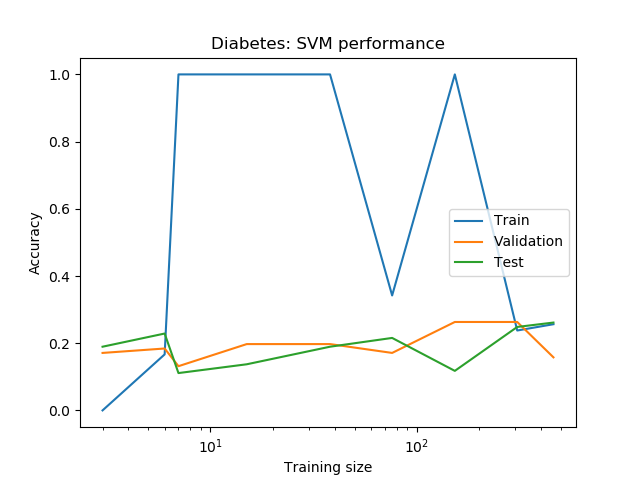
\includegraphics[width=8cm]{diabetes/diabetes_svm_trainingsize.png}

        Here are plots that represent the accuracy with respect to the number of iterations (also done with sklearn's default parameters):

        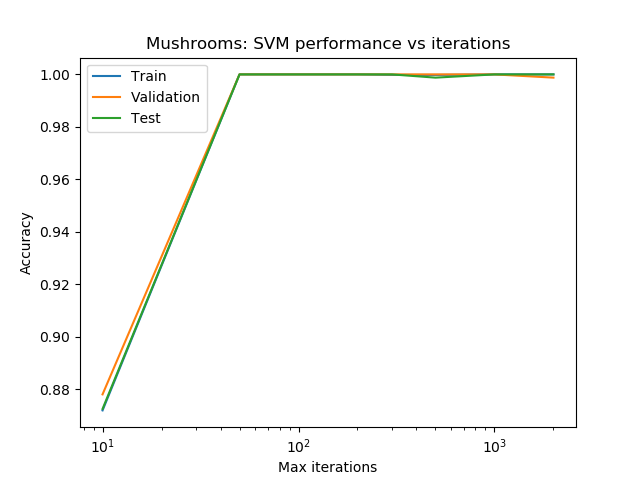
\includegraphics[width=8cm]{mushrooms/mushroom_svm_iterations.png}
        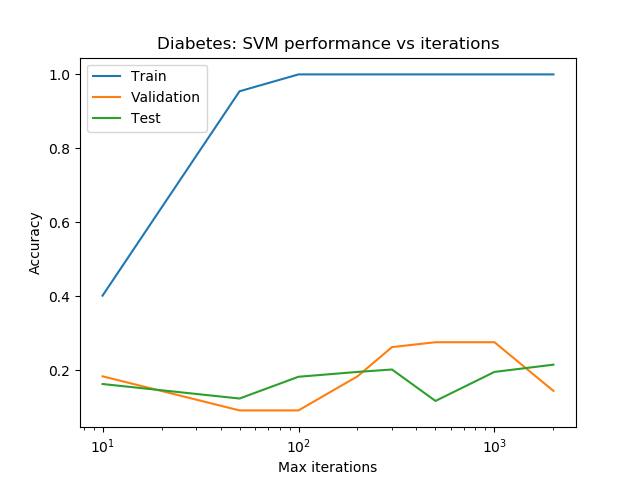
\includegraphics[width=8cm]{diabetes/diabetes_svm_iterations.png}

        \subsection{k-Nearest Neighbors}
        The KNN classifiers were tested with varying K values.

        Here are the KNN plots:

        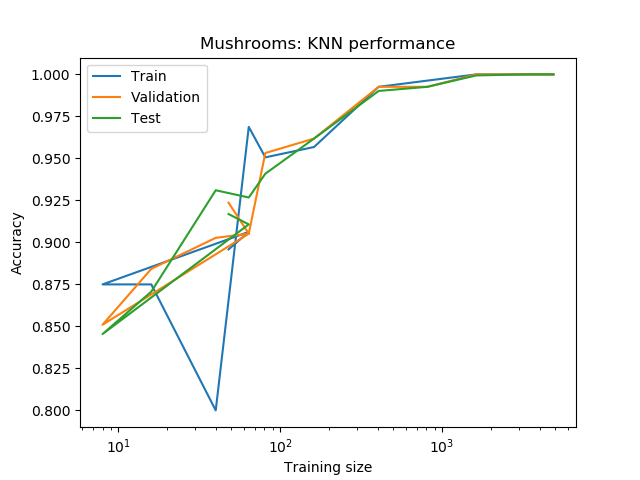
\includegraphics[width=8cm]{mushrooms/mushroom_knn_trainingsize.png}
        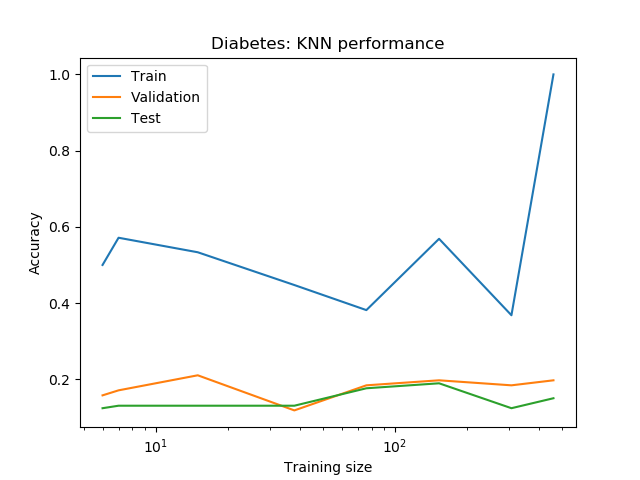
\includegraphics[width=8cm]{diabetes/diabetes_knn_trainingsize.png}

        \section{Analysis}

        Although the datasets had nontrivial sizes (over 700 samples for the diabetes dataset and over 8000 samples for the mushrooms dataset), all the algorithms still ran relatively quickly (each script, which ran some algorithm several times, ran within 1 minute). However, the SVM and neural network relatively took more time than the rest because of their complex architectures. Also, the boosted decision tree relatively took more time since there were two hyperparameters being varied: number of estimators and max depth; the rest of the classifiers had only one hyperparameter varied.

        The accuracy levels for all the classifiers were relatively low for the Diabetes dataset. This could have been due to the relatively small amount of data (768 samples for this dataset versus 8,124 for the Mushroom dataset). Also, more hyperparameter tuning could potentially give better results in this dataset (most of the classifiers involved the tuning of 1 hyperparameter for the sake of efficiency, but given plenty of time, one could use a grid search algorithm with several hyperparameters to find the optimal combination). One trend that is promising, though, is that the accuracy for the training, validation, and test data sharply increase when the last bit of data is added for the boosted and regular decision trees. This leads to the possibility that those two classifiers have a working set of hyperparameters and could give robust results if given more data points.

        For the mushrooms dataset, all the classifiers had accurate performance in the validation and test set when trained with at least 1000 data points. This is because the data was plenty, so even if the model was complex, the large amount of data reduced the error due to variance and allowed the trained data to better generalize to new data. While all models performed well when the amount of data was high, there were insight-providing differences in their performances with less data, which will be discussed below.


        \subsection{Decision Trees}


        Decision trees are very effective at learning the mushroom data even with a relatively
        small training size of 100 examples. This is because the values of the inputs
        are discretized, so there is a relatively small number of input combinations (a few orders
        of magnitude larger than $2^{25}$), so several cases (at least $2^{20}$, a weak lower bound for a decision tree with a max depth of 20) can be learned easily by the branching
        pattern of a decision trees.

        \subsection{Neural Networks}

        The neural networks had very low variance for both datasets.
        A wide range of layers was picked ($[(10,), (5, 10, 5,), (5, 10, 10, 5), (5, 10, 10, 10, 5,)]$),
        so the one with the best results must have been a relatively simple model such as
        the model with one hidden layer of size $10$, allowing the variance to be low.

        \subsection{Boosting}

        Boosting produced much better results than the decision trees. In the cases with less data, the decision
        tree had some overfitting (for example, the validation and testing accuracy would be around 70 percent),
        but boosting, which was designed to overcome this issue of overfitting, resulted in validation
        and testing accuracies of 96 - 97 percent.

        \subsection{Support Vector Machines}

        The support vector machine has a complex model, so more data is needed to provide a high accuracy for it. We can see from the plot in the mushrooms dataset
        that the SVM has a high training accuracy but low validation and testing accuracy for small amounts of data, so more training examples helps to increase the
        validation and testing accuracy. The overfitting can definitely be
        seen in the diabetes accuracy plot, where the training accuracy
        stays around 1.0, while the validation and testing accuracies have low values around 0.2.
        
        A method that could have been used to
        fix the issue of overfitting could have been altering the value of the regularization hyperparameter $C$,
        but this could potentially be computationally intensive, since it would involve grid
        searching on multiple parameters with a computationally expensive model.

        \subsection{k-Nearest Neighbors}

        There was not much of an overfitting problem for this algorithm; there was
        very low variance in the mushrooms dataset. However, there is some overfitting
        in the diabetes dataset, as can be seen in the upshot in the accuracy to 1.0 when the training
        size is larger. Picking a larger value for $K$ could help with this issue (the
        values of $K$ that were tested in this were $1, 2, 3, 4, 5$; possibly increasing
        $K$ to 11 could resolve this issue).

        \section{Sources}

        https://www.kaggle.com/uciml/pima-indians-diabetes-database

        https://www.kaggle.com/uciml/mushroom-classification

    \end{document}